\section{はじめに}
\subsection{背景}
電離圏研究を目的とする短波ドップラー(HFD)の観測データは, 自然科学分野の研究のためオープンデータとして公開され自由な使用が許可されている. \\
現状, 当データの効率的な再利用を推進するためデータのグラフィカルな表示を行う数件のwebアプリケーションが開発されているが, その多くが開発運用やユーザー体験等の観点での問題点を抱えている. \\
現在公開されているwebアプリケーションはデータベースにMySQL, バックエンドにPHP, フロントエンドにHTML/CSS及びJavaScriptを用いて作成されており, 使用されている技術が広範囲に渡ることから開発・保守にかかるコストが高い. \\
またこの点を踏まえフロントエンドとバックエンドの両方にJavaScript(Node.js, React)を用いたアプリケーションも作成されているが, こちらではデータ呼び出しに時間がかかる点やインタラクティブな操作ができないことが課題として挙げられている.

\subsection{本研究の目標}
この課題への対応として既存のアプリケーションから新規アプリケーションを作成するアプローチにより問題点への対応を行うこととした.\\
本研究ではこのwebアプリケーション実装に伴うデータ取得とページのルーティングを通した実装および検証を行う.
\textcolor{red}{やっぱりここら辺でシステムに求められている要件をユーザからの要望リストを元に記述することと、全体において木村さん、藤本君、中村さん、高橋さん、中嶋君がどんな役割を果たしたのか書くことは重要だと思います。今全体が7ページですが、各技術についての記述をもう少し簡潔にすれば(そういうのはChatGPTの方が得意でしょう)もっと全体の計画についての記述にスペースを使えます。}
\textcolor{red}{今のところciteコマンドを用いた参考文献の参照と参照番号の生成がないようです。該当する箇所には参照番号をciteコマンドで挿入しましょう}

\section{使用技術}
\subsection{Next.jsについて}
Next.jsとはVercel社が提供するWebフレームワークである.
JavaScriptのUIライブラリの一つであるReact.jsがベースとなっており, その最大の特徴の一つが多様なページレンダリング手法のサポートである.
このフレームワークは, 開発者がアプリケーションの特定のニーズに応じて最適なレンダリング戦略を選択できるように設計されている. \\
Next.jsのレンダリングオプションには, 一般的なクライアントサイドレンダリング(CSR)の他に, サーバサイドレンダリング(SSR), スタティックジェネレーション(SG)、およびインクリメンタル静的再生成(ISR)が含まれる.\\
2024年現在, バージョン12系以前で用いられていたクライアントサイドでのレンダリングをデフォルトとしたPage Routerとバージョン13系で追加されたサーバーサイドでのレンダリングをデフォルトとしたApp Routerの2種類のRouting手法が存在する.
本研究ではPage Routerを用いることとした.

\subsection{ページレンダリング手法}
\subsubsection{ページレンダリングとは(半分くらいに要約する)}
Webアプリケーションにおいてページレンダリングとは, ウェブサーバーまたはブラウザがHTML/CSS/JavaScriptなどのコードを解釈し, ユーザーのデバイス上で視覚的なページとして表示するプロセスのことである.
プロセス内の各ステップを実行するタイミング等により分類されており, 適切な手法を選定することによりサイトの高速化やユーザ体験の改良, SEOの改善等が期待できる.\\
多くのアプリケーションではServerSideApplicationと呼ばれるサーバーに対して送られたリクエストに対して生成されたHTMLを返す手法や, Ajaxと呼ばれる非同期的な追加リクエストを送ることのできる手法が多く用いられている.\\
しかし現代では仮想DOMと呼ばれる技術を用いることでフォーマンス向上と効率的なUI更新を実現する手法が用いられるようになって来ており, Next.jsでも仮想DOMが使われている.\\
Next.jsの開発元であるVercel社のCEO, Guillermo Rauch氏は "7 Principles of Rich Web Applications" という題の記事を書いており, その中でも第一項目に 'Pre rendered pages are not optional(サーバーがページをレンダリングするのは任意ではない (必須である)。)'と残している. 
このことからもサーバーサイドでレンダリングを行うことでラウンドトリップそのものの回数を削減することはユーザー体験上とても重要であると言えるであろう.
ここではNext.jsで用いられている代表的なレンダリング手法とそのメリット・デメリットについて記す.

\subsubsection{CSR}
CSR(クライアントサイドレンダリング)は, ウェブページのレンダリングをクライアント側(ブラウザ)で行う手法である.
このアプローチでは、サーバーからHTMLの基本骨格とJavaScriptを送信し、クライアント側でHTMLを動的に生成する.\\
CSRはウェブページの内容を動的に更新することが可能で, ユーザーインタラクションに応じて即座にコンテンツを変更できるため, SPA(シングルページアプリケーション)の構築に適している. また, サーバーへのリクエスト回数が減少するためサーバーの負荷を軽減することができる.
しかし初回ロード時にJavaScriptのダウンロードと実行が必要なため, 表示までの時間が長くなる可能性がありSEO対策に不利な点がデメリットとして挙げられる. また, JavaScriptが無効になっている環境ではコンテンツが正しく表示されない可能性がある.\\
CSRのアーキテクチャ図を図\ref{fig:CSR-image}に示す.

\begin{figure}[htbp]
	\begin{center}
		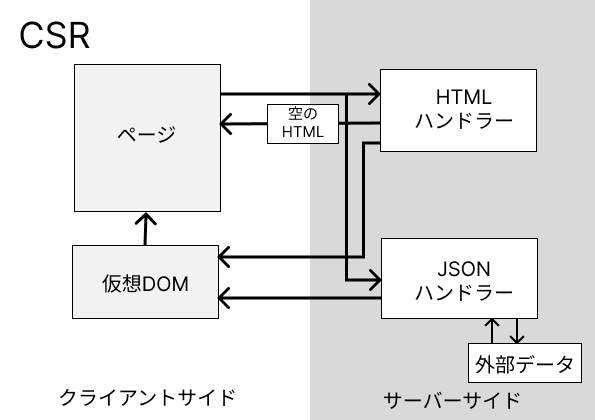
\includegraphics[width=100mm]{./images/CSR.png}
		\caption{CSRのアーキテクチャ}\label{fig:CSR-image}
	\end{center}
\end{figure}

\subsubsection{SSR}
SSR(サーバーサイドレンダリング)はウェブページのレンダリングをサーバー側で行う手法である.
この手法ではユーザーのリクエストに応じてサーバーがHTMLを生成し, 完成したページがクライアントに送信される. \\
SSRはリクエストが起きたタイミングでクライアントサイドと比較して高速なサーバーサイドでHTMLが生成されるため, 初回ページロードの速度を向上させSEO対策に有効である.\\
他にも完成されたHTMLが送信されるためSEOに強い点や, クライアントサイドのJavaScript実行環境に依存しにくい点がメリットである.
しかし, サーバー負荷が大きい点やページ間移動にリロードが伴う点, 後述するSGやISRと比較するとコンテンツの表示に時間が掛かる点等がデメリットとして存在する.\\
SSRのアーキテクチャ図を図\ref{fig:SSR-image}に示す.

\begin{figure}[htbp]
	\begin{center}
		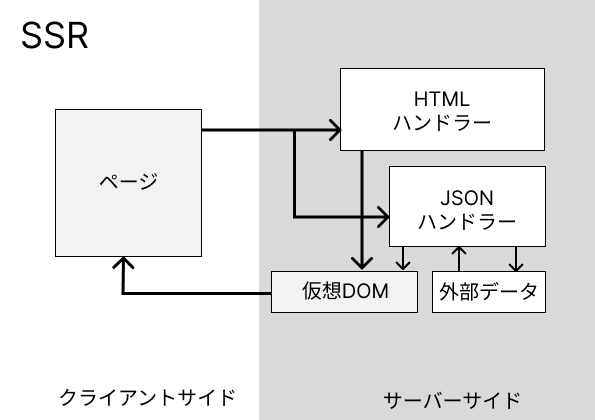
\includegraphics[width=100mm]{./images/SSR.png}
		\caption{SSRのアーキテクチャ}\label{fig:SSR-image}
	\end{center}
\end{figure}
\subsubsection{SG}
SG(スタティックジェネレーション)は, ビルド時に静的なHTMLファイルを生成しておく手法である.
このアプローチではビルド時にすべてのページが静的なHTMLとして生成され, リクエストに応じてそのHTMLが提供される.\\
ビルド時にHTMLが生成されレスポンスの際にはそれを提供するだけのため非常に高速であることがメリットとしてあげられるが, ビルド後の変更が困難なため動的なページ生成には向かないというデメリットが存在する.\\
SGのアーキテクチャ図を図\ref{fig:SG-image}に示す.

\begin{figure}[htbp]
	\begin{center}
		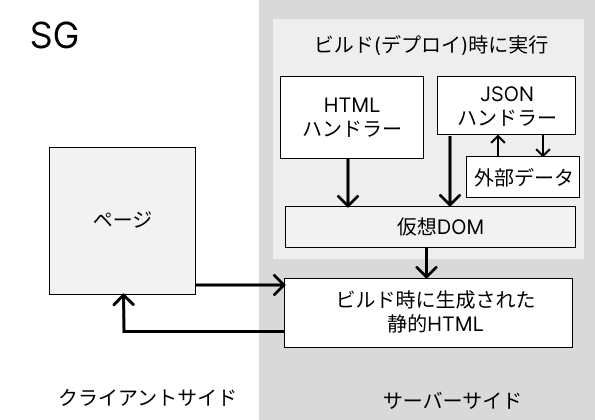
\includegraphics[width=100mm]{./images/SG.png}
		\caption{SGのアーキテクチャ}\label{fig:SG-image}
	\end{center}
\end{figure}

\subsubsection{ISR}
ISR(インクリメンタルスタティックリジェネレーション)は, 静的サイトの生成とサーバーサイドレンダリングを組み合わせた手法である. 
ISRでは, ビルド時に一部のページのみを静的に生成し残りのページはユーザーのリクエストに応じて生成されキャッシュされる. 
これにより, サイトのビルド時間を短縮しつつ動的なコンテンツの提供が可能となる.\\
静的生成と動的生成のバランスが取れパフォーマンスとコンテンツの更新の柔軟性が両立されているメリットがあるが, 再生成後初回リクエスト時のオーバーヘッドが大きく読み込みに時間がかかってしまう場合があるというデメリットが存在する.\\
ISRのアーキテクチャ図を図\ref{fig:ISR-image}に示す.

\begin{figure}[htbp]
	\begin{center}
		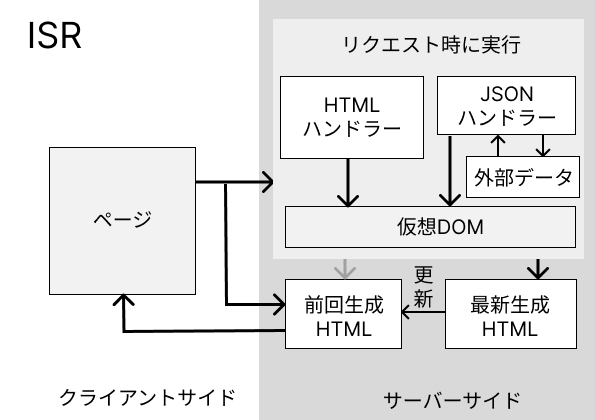
\includegraphics[width=100mm]{./images/ISR.png}
		\caption{ISRのアーキテクチャ}\label{fig:ISR-image}
	\end{center}
\end{figure}

\subsubsection{Next.jsにおけるページレンダリング}
Next.jsのページレンダリングは主にページコンポーネントのライフサイクルとデータ取得方法に依存する特徴があり, それらのレンダリング手法をページごとに異なる方法で適用できる柔軟性にも優れている.\\
例として一部のページはSSRを使用して動的にデータを取得を行い、他のページはSGを使用して静的に生成することも可能である.
このような柔軟性により開発者はパフォーマンス, SEO, ユーザーエクスペリエンスのバランスを取りつつ, アプリケーションの特定の要件に合わせて最適なレンダリング戦略を選択できる.
これにより, 開発者はより高速で対話的なウェブアプリケーションを構築することができ, 最終的にはユーザーに優れた体験を提供することが可能となる.

\subsection{スクレイピングについて}
このアプリケーションは, 各観測所にて観測されたデータを素のディレクトリ構造のまま公開されている既存のアプリケーションからデータをスクレイピングしてきて再描画を行うものである.
スクレイピングとはwebアプリケーションからHTMLデータをクローラによって取得し、必要とされる情報を抽出するする技術のことである.\\
スクレイピングの際には取得元のサイトの規約に乗っ取る義務がある.
今回の場合は取得先のデータがOSS化されていることと学術目的として取得先の団体からの許可を得ていることから, 過剰な負荷がかからない範囲内での利用が可能であると判断した.\\
実装にはライブラリとしてSuperagentとCheerioを用いてNext.js上でTypeScript関数として実装した.\\
一般的にスクレイピングのような外部サイトにアクセスする場合はCORS(Cross-Origin Resource Sharing)エラーに注意する必要がある.
CORSエラーは, ウェブページがクライアントサイドで異なるオリジン(異なるドメイン, プロトコル, またはポート)からのリソースにアクセスしようとしたときに発生するセキュリティ上の問題である.\\
ウェブサイト(当アプリケーション)が異なるドメインの別のウェブサイト(スクレイピング先)にホストされているAPIからデータを取得しようとする場合, ブラウザはこのアクセスを同一オリジンポリシーによりブロックしてしまう場合がある.
しかし今回の場合はレンダリングをサーバーサイドで行いクライアント側で直接アクセスされないためNext.jsというフレームワーク上でデータのスクレイピングを行ってもCORSエラーは発生しない.

\section{アプリケーション設計と実装方法}
\subsection{実装の要件}
本研究ではアプリケーション実装のうち外部データの取得とページの描画を主体としている.
そのためUX向上を目的とした,データフェッチからの画面描画速度の高速化を目標に設定した.\\
今回作成するアプリケーションのうち, webスクレイピングを伴うページは大きく分けて以下の2つである.\\
\begin{quote}
	\begin{itemize}
		\item 波形データの検索ページ
		\item 波形の描画ページ
	\end{itemize}
\end{quote}
これらのページの実装を行い、ビルド時間とスクレイピングのリクエスト数の2軸から最適化を行うものとした.

\subsection{スクレイピングに用いた関数}
今回実装したスクレイピング関数は大きく2つあり, 1つは指定した日時・観測所の周波数のCSVデータをJSON化して取得するもの, もう1つは存在するデータの一覧を取得するものである.
スクレイピング先のアプリケーションでは観測所・年度・日時の順にネストされたパスから周波数のデータを取得可能である. 
1つめの関数ではURLで具体的なデータの所在ページを指定した上でスクレイピングした.
2つめの関数では存在するページの一覧化のため観測所のひとつ上の階層から子要素となるページを再帰的に全探索する形でスクレイピングし整形を行った.

\subsection{レンダリング設計}
次にレンダリング設計について述べる.
以下の2パターンの設計で実装を行い、ビルドにかかった時間を比較し考察することとした.
\begin{quote}
	\begin{enumerate}
		\item ISRを用いる方法
		\item SGとSSRを用いる方法
	\end{enumerate}
\end{quote}
\subsubsection{ISRを用いる方法}
1つ目の手法はISRを用いた実装である.
この手法はビルドの際に一括でスクレイピング処理を完結させて静的なサイトを生成するものである.\\
実装方法はgetStaticPathsと呼ばれる関数内でディレクトリ一覧をスクレイピングし静的にビルドするページを確定させた上で, getStaticPropsという関数でそれら一つ一つのページの波形データを取得してビルドを行う.\\
またISR技術を用いて再ビルドのタイミングを制御することにより, 一定期間ごとに新しく追加されたデータも取得できるようにさせることができるようにする.

\begin{figure}[htbp]
	\begin{center}
		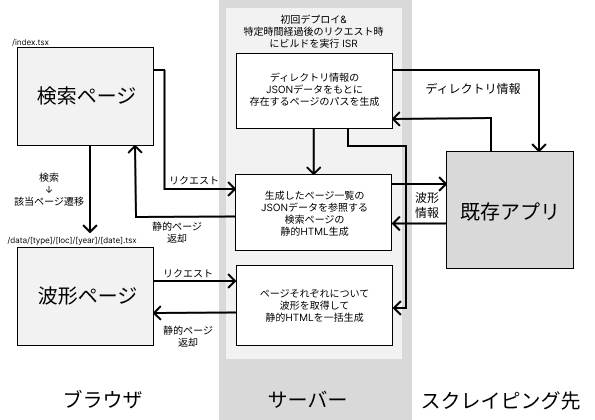
\includegraphics[width=100mm]{./images/app/ISRver.png}
		\caption{ISRを用いた場合の設計}\label{fig:ISR-arc}
	\end{center}
\end{figure}

\subsubsection{SGとSSRを用いる方法}
2つ目の手法はSGとSSRを併用させる方法である.
この手法ではディレクトリの取得と波形データの取得をそれぞれSG・SSRをもちいて分離させる方法である.
実装方法はgetStaticPropsを用いて検索ページに存在するパスを静的に生成し, getServerSidePropsを用いて各ページでリクエストされた際に動的に波形データを返すというものである.

\begin{figure}[htbp]
	\begin{center}
		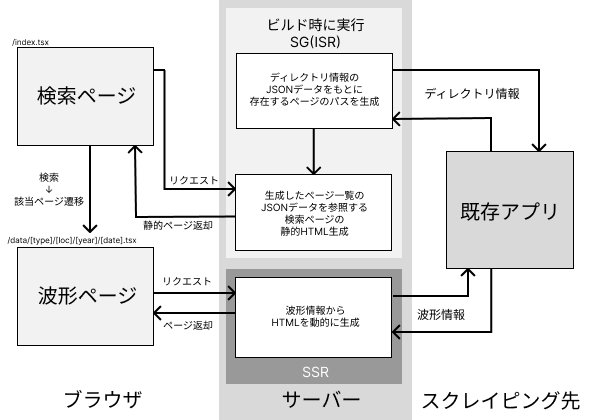
\includegraphics[width=100mm]{./images/app/SG-SSRver.png}
		\caption{SGとSSRを併用した場合の設計}\label{fig:SG-SSR-arc}
	\end{center}
\end{figure}

\subsection{実行環境}
今回の実行環境としたPCを表\ref{table:zikkoukannkyo}に示す.\\
また使用したパッケージのバージョンを表\ref{table:version}に示す.

\begin{table}[hbtp]
	\caption{実行環境}
	\label{table:zikkoukannkyo}
	\centering
	\begin{tabular}{lcr}
		\hline
		名称      & MacBookPro    \\
		CPU     & Apple M1 Max  \\
		メモリ     & 32GB          \\
		コマンドシェル & zsh (v1.85.1) \\
		\hline
	\end{tabular}
\end{table}

\begin{table}[hbtp]
	\caption{パッケージのバージョン}
	\label{table:version}
	\centering
	\begin{tabular}{lcr}
		\hline
		名称         & バージョン   \\
		\hline \hline
		Node.js    & 18.12.0 \\
		Next.js    & 13.0.6  \\
		TypeScript & 4.9.4   \\
		
		\hline
	\end{tabular}
\end{table}


\section{実装結果}
\subsection{データ取得}
今回の実装では2種類いずれの方法でもデータを取得する事ができた.\\
図\ref{fig:search-page-image}と図\ref{fig:wave-page-image}にデータを取得してそのJSONデータをブラウザ上に表示した様子を示す.

\begin{figure}[htbp]
	\begin{center}
		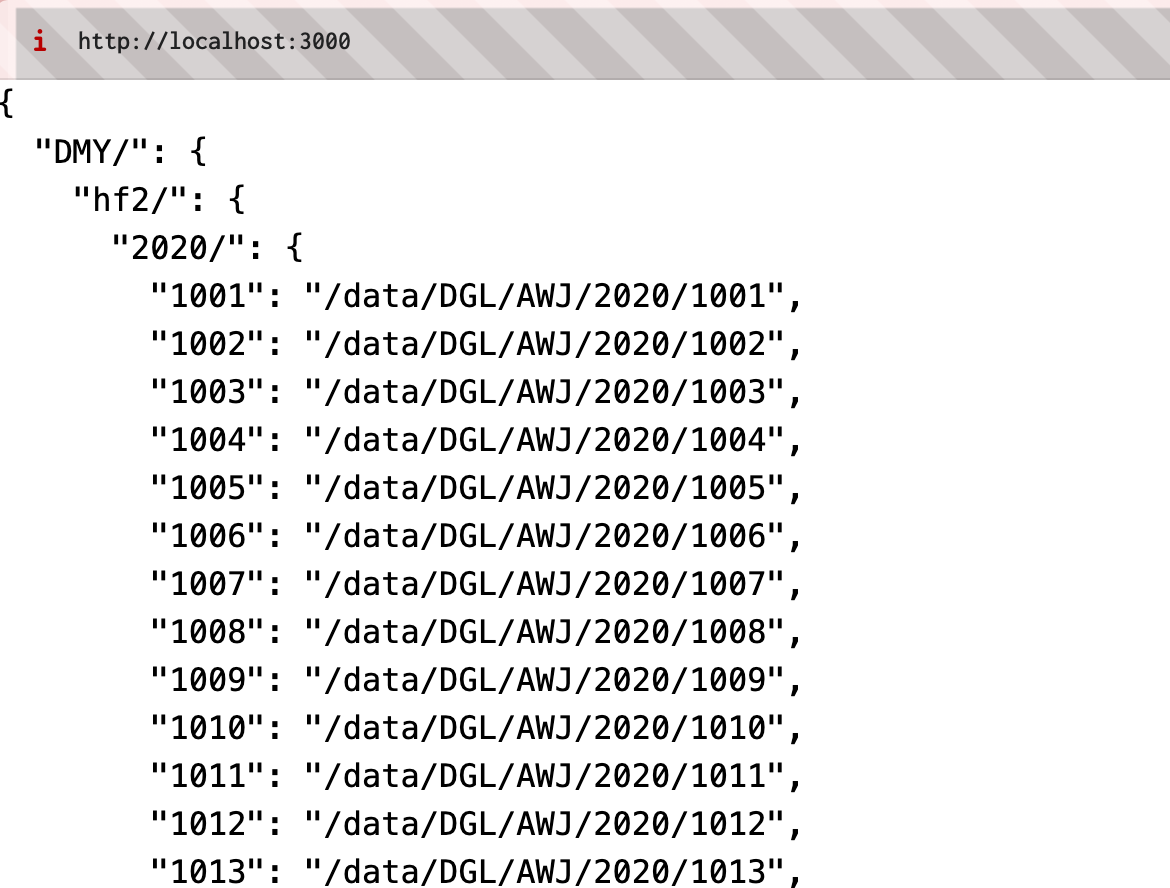
\includegraphics[width=100mm]{./images/search-page-image.png}
		\caption{検索ページでデータ取得している様子}\label{fig:search-page-image}
	\end{center}
\end{figure}

\begin{figure}[htbp]
	\begin{center}
		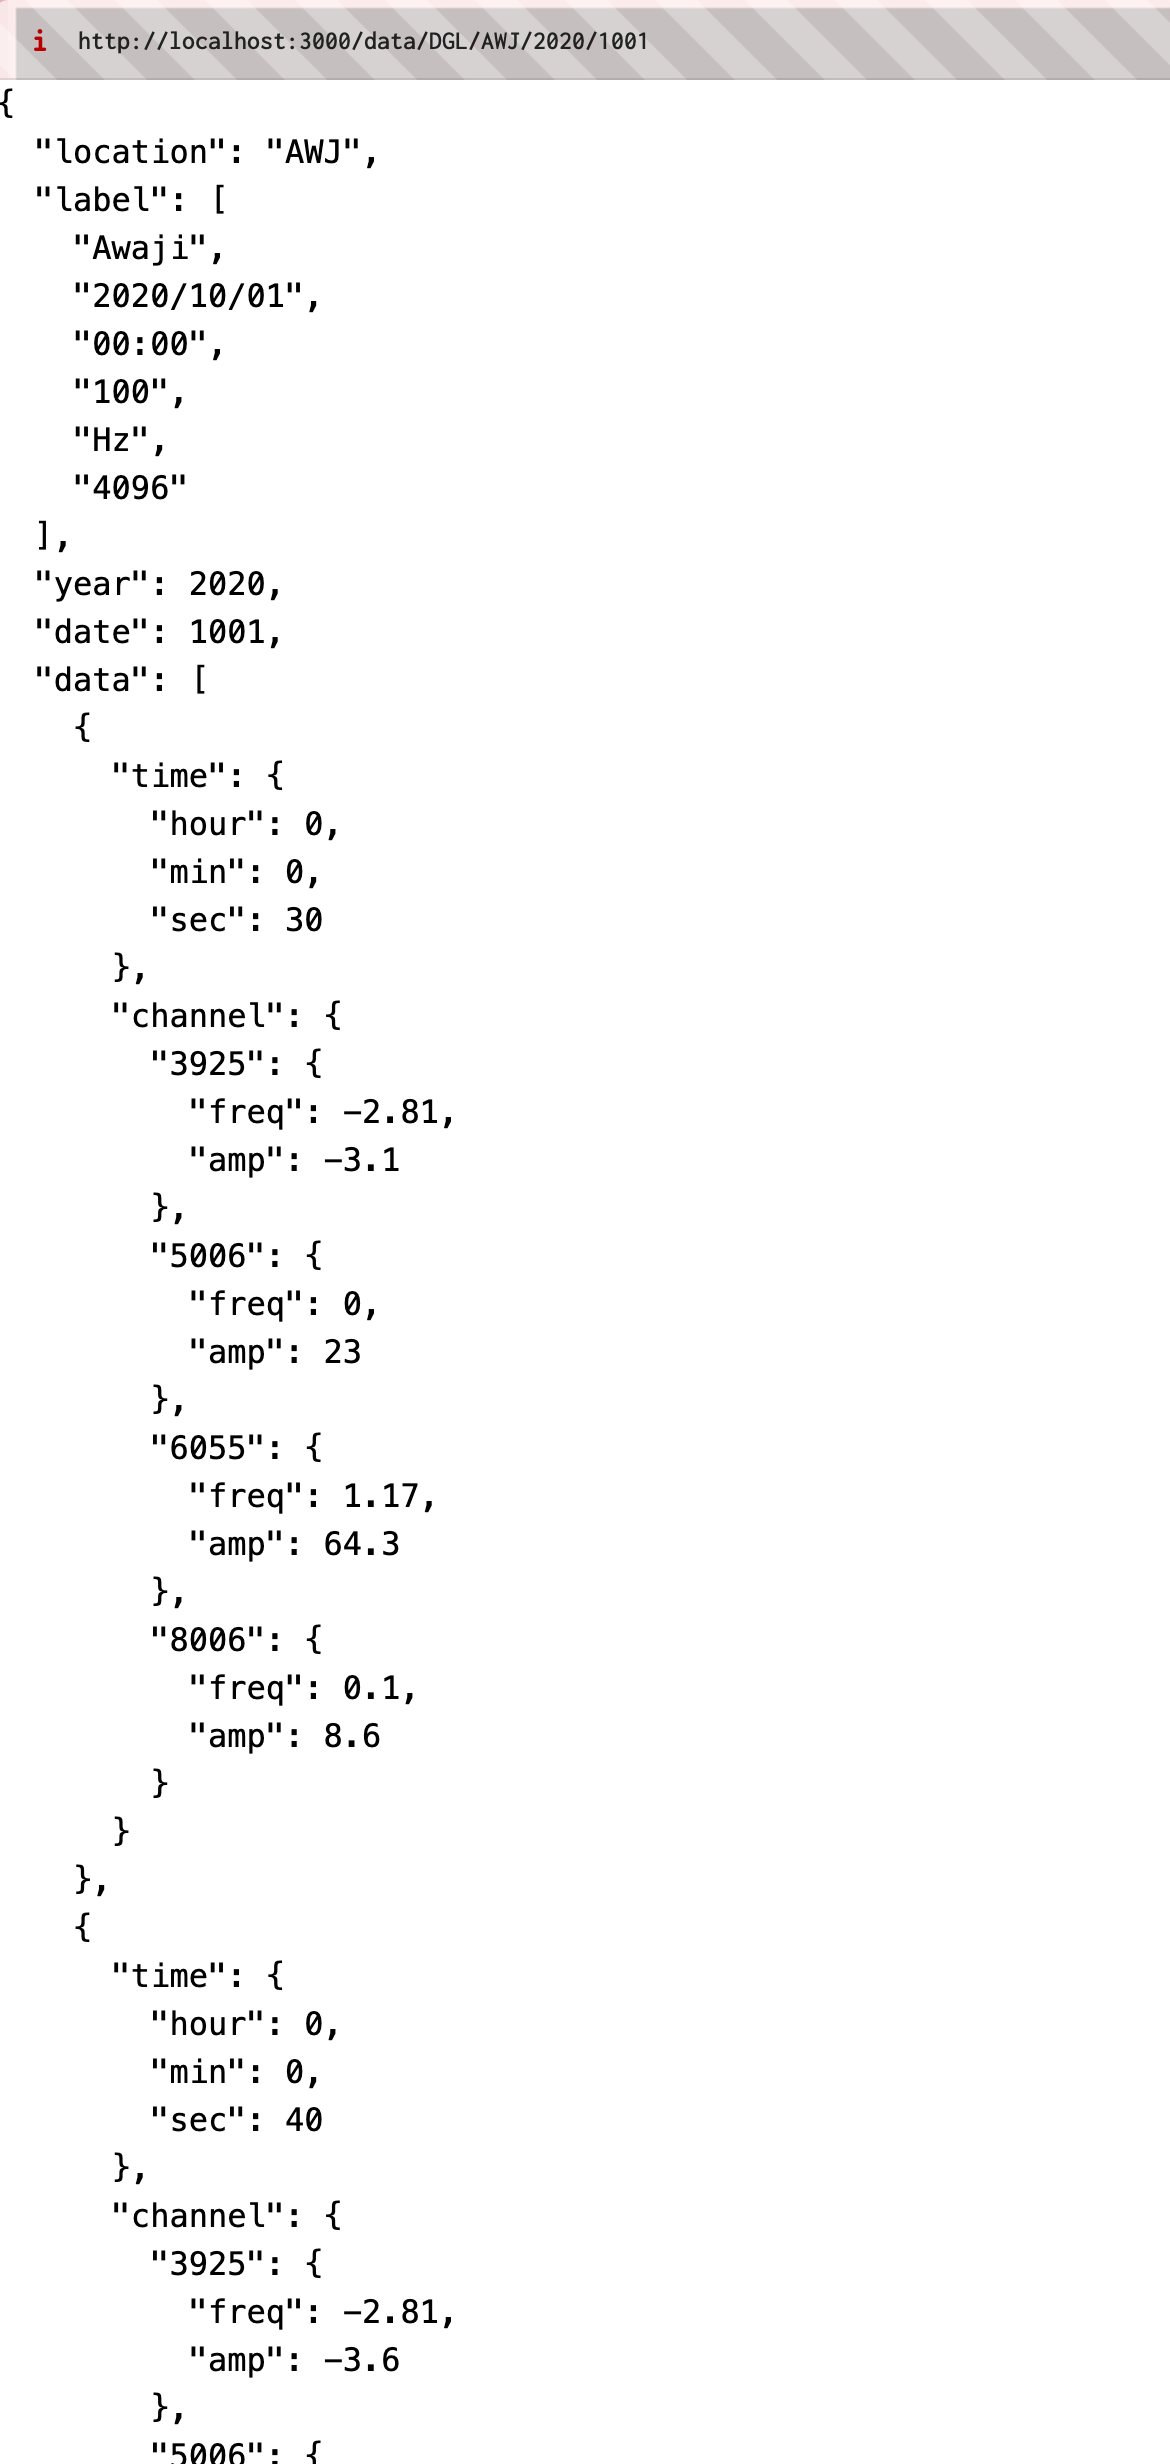
\includegraphics[width=100mm]{./images/wave-page-image.png}
		\caption{波形ページでデータ取得している様子}\label{fig:wave-page-image}
	\end{center}
\end{figure}


\subsection{スクレイピング関数の実行時間}
実装した2つの関数の実行時間を示す.
なお実行時間計測にはperformance.now()メソッドを用い, 関数の実行前後の時間差から計測している.

\subsubsection{scrapeWaveData}
この関数は, 引数で渡したデータ形式, 観測所名, 年, 日時から観測データのCSVデータを取得しJSON形式に変換するものである.
実行時間を表\ref{table:scrapeWaveData}に示す

\begin{table}[hbtp]
	\caption{scrapeWaveDataの実行時間}
	\label{table:scrapeWaveData}
	\centering
	\begin{tabular}{lcr}
		\hline
		回数  & 実行時間(ms) \\
		\hline \hline
		1回目 & 1435     \\
		2回目 & 1166     \\
		3回目 & 1054     \\
		4回目 & 997      \\
		\hline
		平均  & 1163
	\end{tabular}
\end{table}

結果としておよそ1秒でデータの取得ができることが確認できた.

\subsubsection{scrapeDirectory}
この関数は, 引数で渡したURL配下に存在するページを再帰的に全探索し, ディレクトリ名をキーとするネストされたオブジェクトとして返す.
実行時間を表\ref{table:scrapeDirectory}に示す.

\begin{table}[hbtp]
	\caption{scrapeDirectoryの実行時間}
	\label{table:scrapeDirectory}
	\centering
	\begin{tabular}{lcr}
		\hline
		回数  & 実行時間(ms)   \\
		\hline \hline
		1回目 & 319411     \\
		2回目 & 325276     \\
		3回目 & 263359     \\
		4回目 & 261885     \\
		\hline
		平均  & 292482.75
	\end{tabular}
\end{table}

結果として実行には300秒前後かかることが確認できた.

\subsection{静的ビルドの実行時間の比較}
ISRを用いる手法とSGとSSRを併用する方法との2パターンでビルドを実行し, ビルドログに出た実行時間を示す.
\subsubsection{ISRを用いる方法}
ISR(SG)を用いて, ビルド時に存在するパスを生成した後各ページまでを静的に生成する方法を用いた場合のビルドログを図\ref{fig:ISR-build}に示す.

\begin{figure}[htbp]
	\begin{center}
		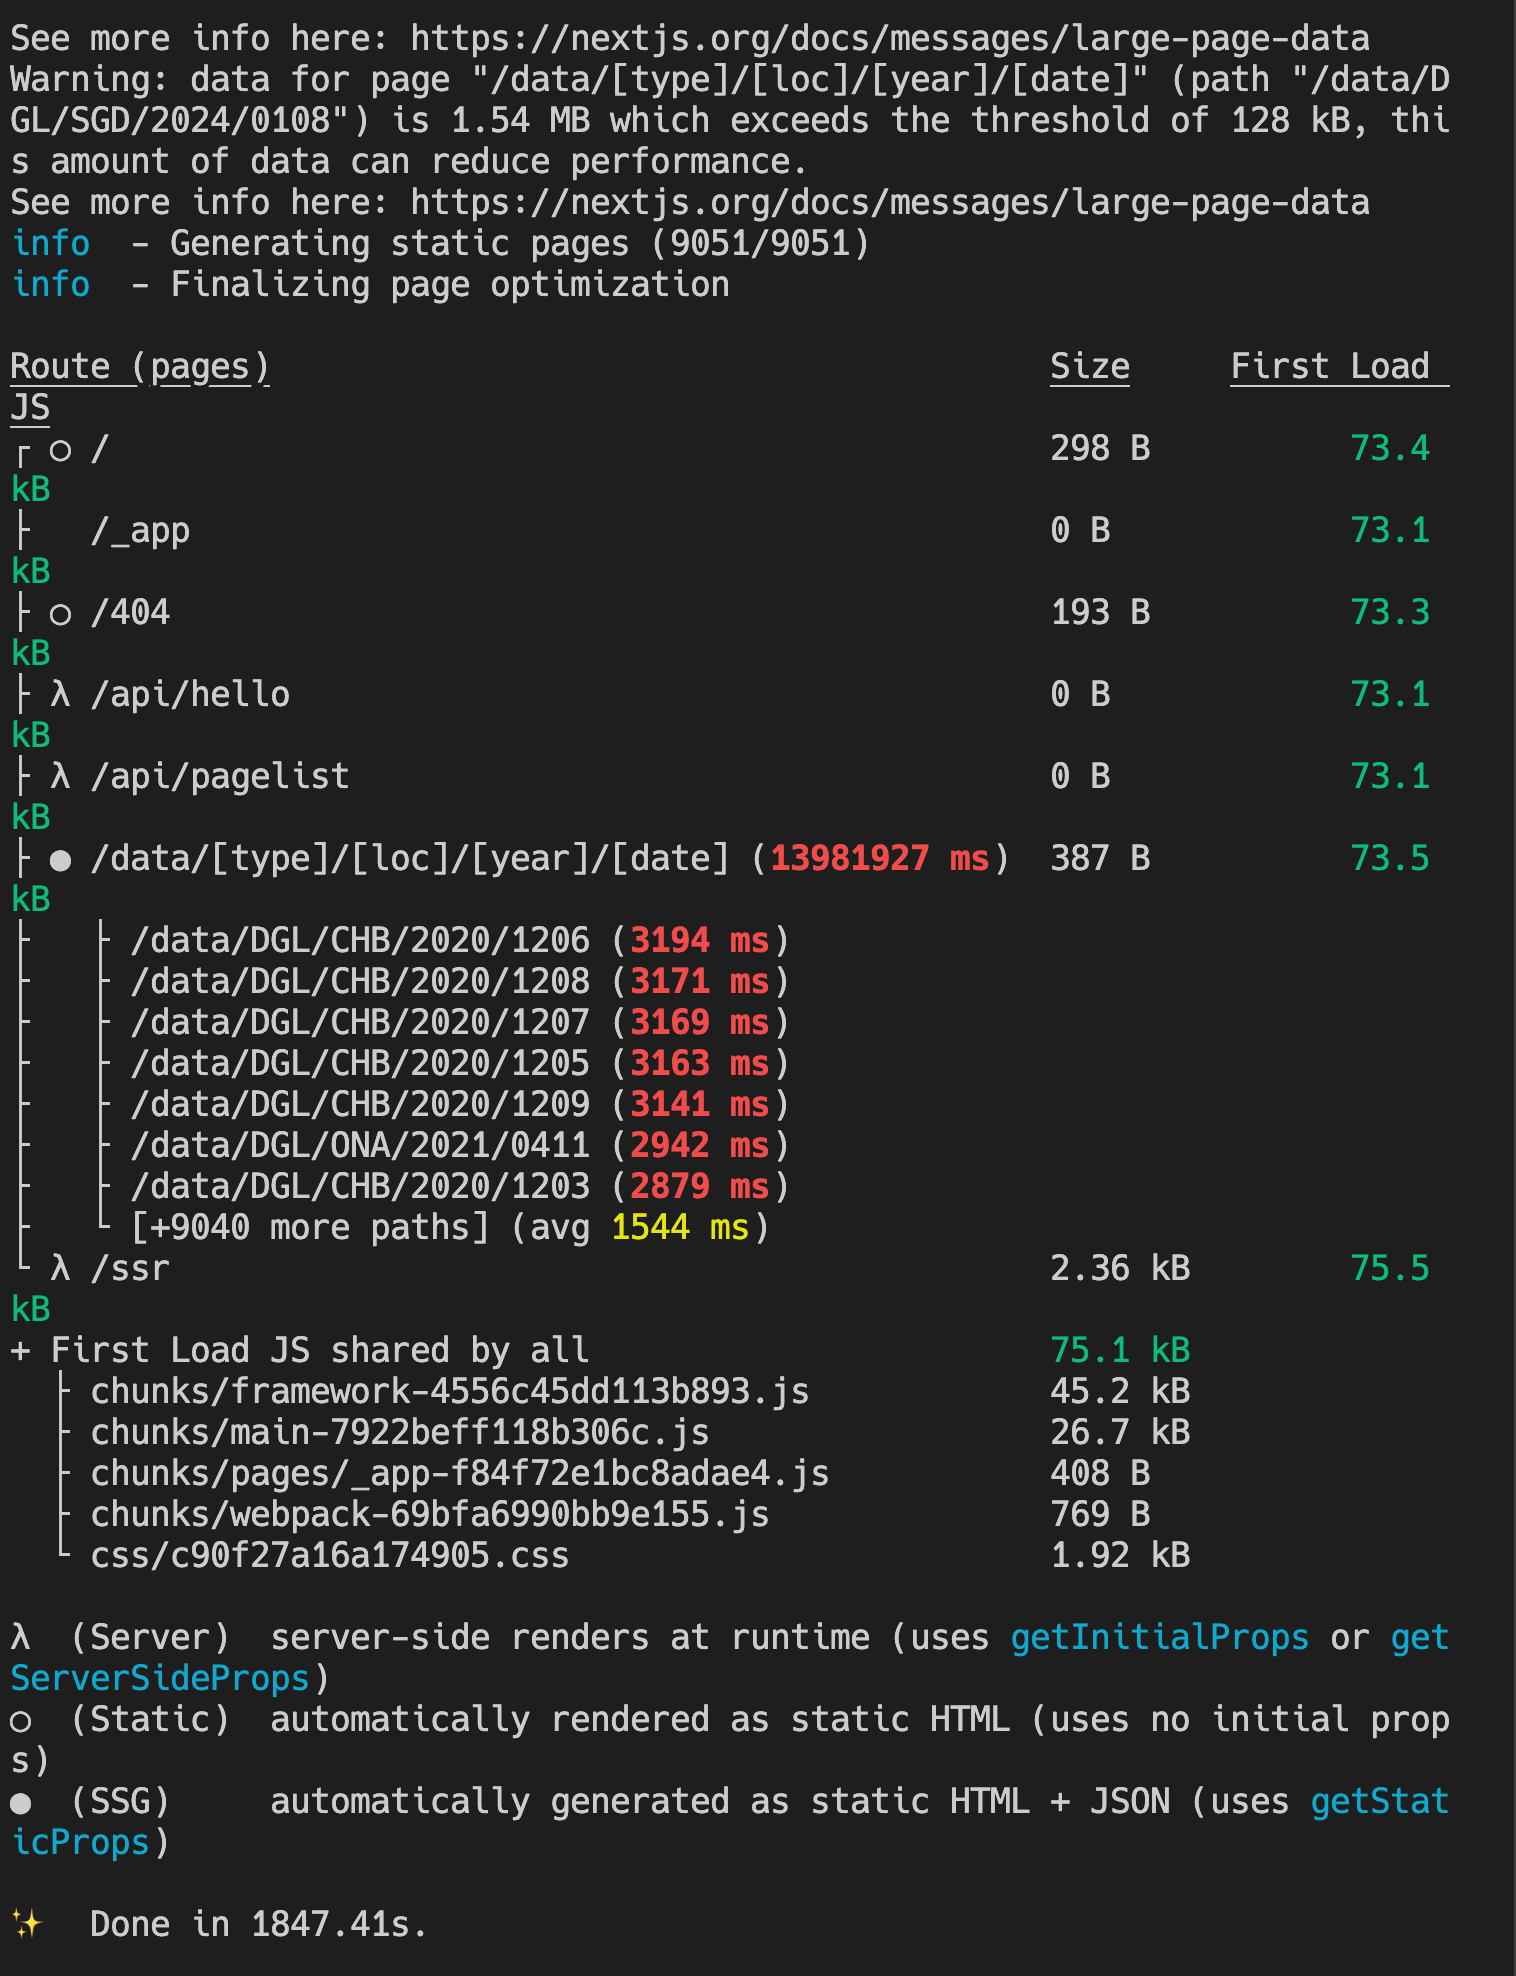
\includegraphics[width=100mm]{./images/ISR-log.png}
		\caption{ISR(SG)を用いた際のビルドログ}\label{fig:ISR-build}
	\end{center}
\end{figure}

実行結果からビルド時間は1847秒であることが確認できる.

\subsubsection{SGとSSRを用いる方法}
SGとSSRを併用して, ビルド時には存在するパスのみを静的に生成しておき,各ページはアクセスされた際に動的に生成した場合のビルドログを図\ref{fig:SG-SSR-build}に示す.

\begin{figure}[htbp]
	\begin{center}
		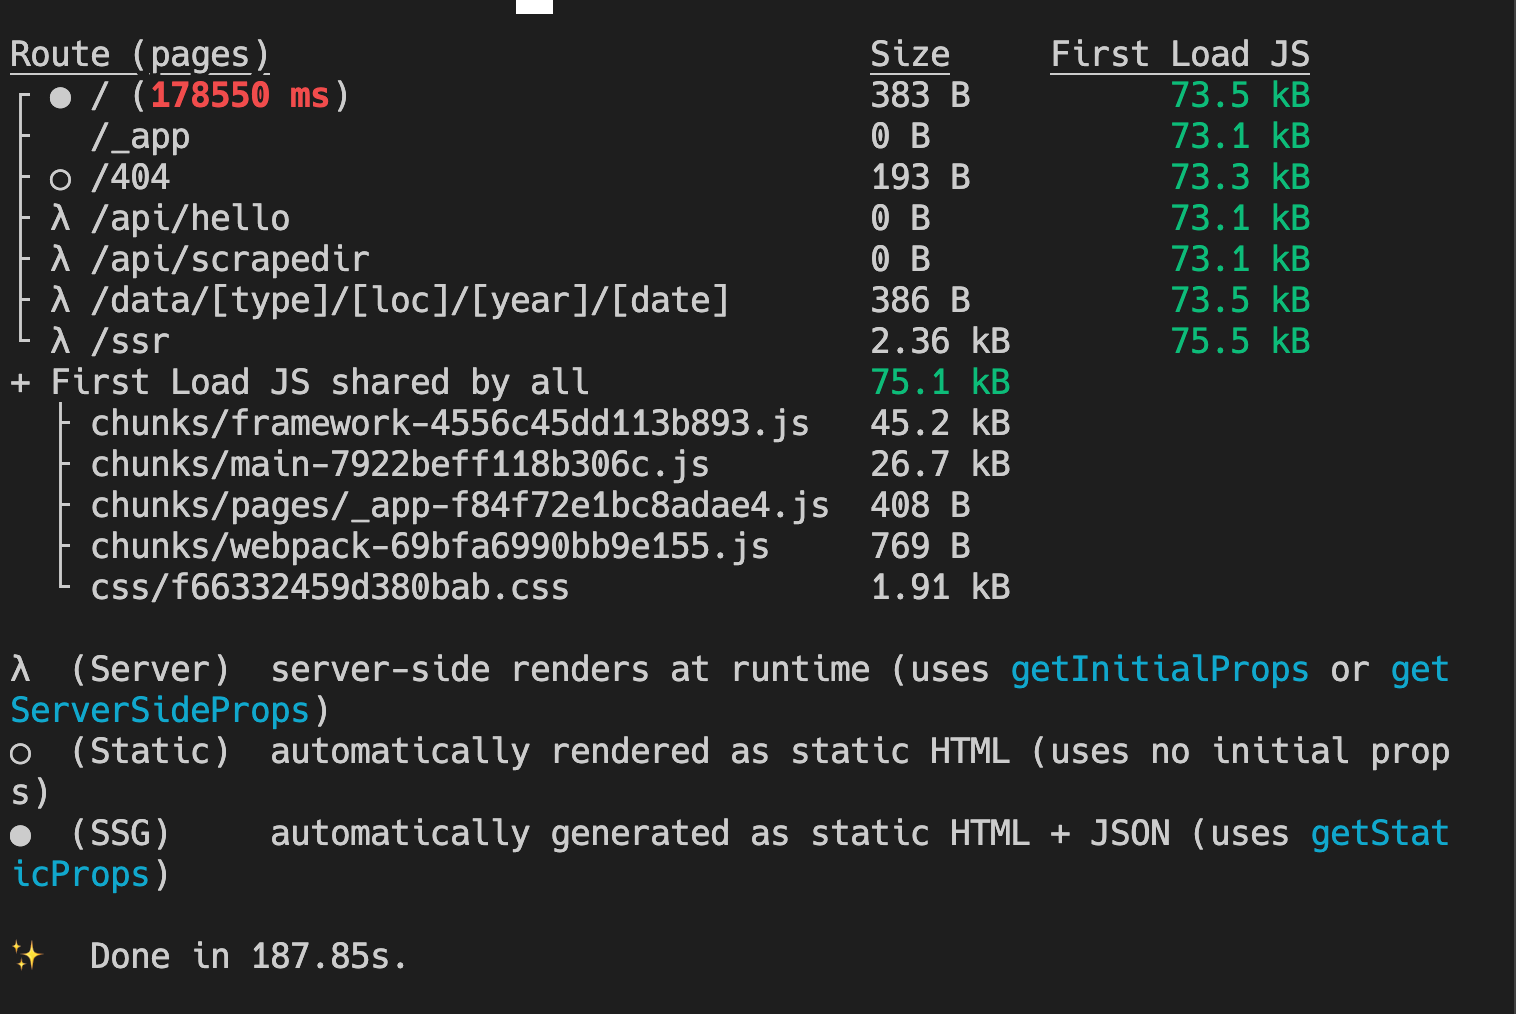
\includegraphics[width=100mm]{./images/SGandSSR-log.png}
		\caption{SGとSSRを併用した場合のビルドログ}\label{fig:SG-SSR-build}
	\end{center}
\end{figure}

実行結果からビルド時間は1847秒であることが確認できる.

\section{考察}
\subsection{スクレイピングの実行結果について}
スクレイピングの実行結果より, ディレクトリ情報取得は波形データの取得と比較して時間がかかることが確認できる.
これは波形データの取得は一度のページアクセスで済むのに対して, ディレクトリ情報の取得はディレクトリの全探索であり複数回のページアクセスの必要が出てくるためであると考えられる.

\subsection{ビルドの実行結果について}
ビルド時間を比較した際にISRを用いた場合はSGとSSRを併用した場合に対して約10倍かかってしまうことが見て取れる.

\subsection{ビルド方法の選定}
これらの結果を踏まえて当アプリケーションでのビルド方法を選定していく.\\
ISR生成時間に約30分かかってしまうことが確認できた. ISRの仕様として設定した定期時間後の初回アクセス時にビルドが実行されその実行時間がオーバーヘッドとして存在するため, 初回アクセス者に30分間の待機時間が必要である.
これはユーザー体験面において適当ではない.\\
対してSGとSSRを用いた場合にはデータのページに移行する際に約1秒のスクレイピング時間がかかる. 
ページ描画には事前に生成されている静的なデータを返すISRと比較して時間がかかってしまうがオーバーヘッドの問題を踏まえれば許容範囲である.
SGのデメリットとして動的なページ生成に弱い点が挙げられる.
しかし今回のアプリケーションではスクレイピング元のサイトでデータが追加されるのが一日に数回であることから再取得(再ビルド)すべきタイミングは一日に数回程度と想定される.
この場合はGitHub Actions等のCI/CDツールを用いてホスティング先での規定時間ごとの再ビルドを行うことで対応可能であると考察する.\\
CI/CDツールを用いた再ビルドはISRを用いる方法をSG単体を用いる方法と置き換えることでも実現可能ではあるが, GitHub Actionsの料金がジョブの実行時間に依存しているためビルドに過剰な時間がかかる方法は適切ではない.\\
これらの理由をもとに本研究ではSGとSSRを併用させて実装することが現状において最適な手法であると結論づけた.

\subsection{結果を踏まえての追加仮説}
本実験の結果よりSGとSSRを併用する方法が適切であると結論づけた.
しかしこの選択をした場合にデータページへアクセスした際にSSRで実行されるデータフェッチに約1秒かかってしまう点がUX上の課題点として挙げられる.\\
これに対してプリフェッチやを活用することでより高速化が望めるのではないかと再仮説を立てた.\\
プリフェッチとは次にアクセスすると考えられるページのデータを事前に取得しておく技術のことを指す.\\
Next.jsにはNextLinkという機能があり, 現在表示されているページ上にある遷移リンクの情報をプリフェッチしておくことが可能である.
当アプリケーションでの主要なユースケースとして次のフローが考えられる.\\
\begin{enumerate}
	\item データの検索ページにアクセスする.
	\item データを検索してリンクから任意のデータページにアクセスする.
\end{enumerate}
この仮説はフロー上でデータの検索ページにアクセスした後任意のデータページヘ遷移するリンクを表示した時点でプリフェッチを行っておくことで, 実際にアクセスされた後にデータを取得する以上の高速化が望めるのではないかというものである.
Next.jsのドキュメントや有志による技術ブログを調査をした所によるとSSRの際に用いられるgetServerSidePropsによるトップレベルでのデータ取得に関してはNextLinkによるプリフェッチが実行されない様であった.
この場合クライアントサイドでのデータ取得を行い次ページのプリフェッチを可能にした方がユーザーの体感上高速化される可能性がある.\\
また, useSWRと呼ばれるデータ取得のためのReact Hooksライブラリを適切に活用することにより, キャッシュ戦略とプリフェッチを最適化できる事も考えられる.\\
これら仮説に対しては実際に実装してみての検証が必要であり調査する価値は十分あるのではないかと考える.

\section{おわりに}
本研究では電離圏研究を目的とする短波ドップラーの観測データをスクレイピングして再描画するアプリケーションでのレンダリング戦略に関して, 調査と検証を行った.\\
この研究結果及び実装に適切なUI実装を行うことで, 高速でUX的観点上優れたアプリケーションの作成が可能であると考える.\\
また考察時に述べた追加仮説に関しても調査の上導入することによりUX向上の観点で有益な実装となるのではないだろうか.
\textcolor{red}{ユーザからの要望に応えてどのように変更したのかを、もう一度ユーザからの要望を参照しながら本研究の達成度を示しましょう}

\begin{thebibliography}{99}
	\bibitem{no1}
	富家和樹, サービスに応じたUXの設計とページレンダリング手法の実装, 電子制御工学科卒業研究論文集, 北九州工業高等専門学校, 2022
	\bibitem{no2}
	仲純平, 短波ドップラーデータ公開用Webアプリケーションの開発, 特別研究公開発表会, 北九州工業高等専門学校, 2022
	\bibitem{no3}
	手島拓也 吉田健人 高林佳稀, TypeScriptとReact/Next.jsでつくる実践Webアプリケーション開発, 技術評論社, 東京, 2022
	\bibitem{no4}
	ソシオメディア株式会社 上野学 藤井幸多, オブジェクト指向UIデザイン 使いやすいソフトウェアの原理, 技術評論社, 東京, 2020
	\bibitem{no5}
	伊原力也 小林大輔 桝田草一 山本怜, Webアプリケーションアクセシビリティ 今日から始める現場からの改善, 技術評論社, 東京, 2023
	\bibitem{no6}
	Vercel, Next.js by Vercel - The React Framework, https://nextjs.org, (参照2024-1-20)
	\bibitem{no7}
	Vercel, SWR, https://swr.vercel.app/ja, (参照2024-1-20)
	\bibitem{no7}
	Guillermo Rauch, 7 Principles of Rich Web Applications, https://rauchg.com/2014/7-principles-of-rich-web-applications, (参照2024-1-20)
	
\end{thebibliography}